\documentclass[tikz,border=8pt]{standalone}

\usetikzlibrary{
  arrows.meta,
  backgrounds,
  calc,
  fit,
  positioning
}

\definecolor{DataBlue}{HTML}{2F6F9F}
\definecolor{DataFill}{HTML}{EAF3F8}
\definecolor{UserGreen}{HTML}{2F7F5F}
\definecolor{UserFill}{HTML}{EDF7F1}
\definecolor{TargetOrange}{HTML}{B8642F}
\definecolor{TargetFill}{HTML}{FFF1E8}
\definecolor{JudgePurple}{HTML}{7456A6}
\definecolor{JudgeFill}{HTML}{F2EEF8}
\definecolor{StageFill}{HTML}{F7F7F7}
\definecolor{StageBorder}{HTML}{B8B8B8}
\definecolor{Ink}{HTML}{2B2B2B}
\definecolor{Muted}{HTML}{666666}

% Stage layout uses top-left origins. Content inside a stage is local to that
% stage, so spacing changes stay local instead of shifting the full figure.
\def\decompX{-1.55}
\def\decompY{1.42}
\def\decompW{8.35}
\def\decompH{3.22}
\def\convX{7.05}
\def\convY{1.96}
\def\convW{11.10}
\def\convH{4.36}
\def\judgeX{18.55}
\def\judgeY{1.48}
\def\judgeW{6.26}
\def\judgeH{3.20}
\def\handoffY{0.05}
\def\traceY{-2.95}

\newcommand{\stageBackground}[3]{%
  \coordinate (#1NW) at (0,0);
  \coordinate (#1SE) at (#2,-#3);
  \node[stage, inner sep=0pt, fit=(#1NW) (#1SE)] (#1) {};
}

\newcommand{\robotAt}[4]{%
  \begin{scope}[shift={(#1,#2)}]
    \draw[draw=#3, fill=#4, rounded corners=2pt] (-0.38,-0.28) rectangle (0.38,0.32);
    \draw[draw=#3, fill=#4, rounded corners=1pt] (-0.54,-0.12) rectangle (-0.38,0.14);
    \draw[draw=#3, fill=#4, rounded corners=1pt] (0.38,-0.12) rectangle (0.54,0.14);
    \draw[draw=#3, line width=0.8pt] (0,0.32) -- (0,0.56);
    \draw[draw=#3, fill=#4, rounded corners=1pt] (-0.10,0.56) rectangle (0.10,0.70);
    \fill[#3] (-0.15,0.08) circle (1.3pt);
    \fill[#3] (0.15,0.08) circle (1.3pt);
    \draw[draw=#3, line width=0.65pt] (-0.16,-0.13) -- (0.16,-0.13);
  \end{scope}
}

\newcommand{\drawRobotActor}[6]{%
  \coordinate (#1) at (#2,#3);
  \robotAt{#2}{#3}{#4}{#5}
  \node[align=center, font=\sffamily\scriptsize, text=#4] at ($(#1)+(0,-0.48)$) {#6};
}

\newcommand{\drawSourceDocument}[3]{%
  \begin{scope}[shift={(#2,#3)}]
    \coordinate (#1NW) at (-0.78,1.09);
    \coordinate (#1SE) at (0.78,-1.09);
    \coordinate (#1East) at (0.78,0.08);
    \draw[draw=Ink, fill=white, rounded corners=1pt] (#1NW) rectangle (#1SE);
    \draw[draw=Ink, fill=StageFill] (0.47,1.09) -- (0.78,0.78) -- (0.78,1.09) -- cycle;
    \node[font=\sffamily\scriptsize\bfseries, align=center] at (0,0.94) {AITA post};
    \draw[draw=Muted, line width=0.40pt] (-0.55,0.61) -- (0.48,0.61);
    \draw[draw=Muted, line width=0.40pt] (-0.55,0.45) -- (0.36,0.45);
    \draw[draw=Muted, line width=0.40pt] (-0.55,0.23) -- (0.50,0.23);
    \draw[draw=Muted, line width=0.40pt] (-0.55,0.07) -- (0.42,0.07);
    \draw[draw=Muted, line width=0.40pt] (-0.55,-0.15) -- (0.46,-0.15);
    \draw[draw=Muted, line width=0.40pt] (-0.55,-0.31) -- (0.30,-0.31);
    \draw[draw=Muted, line width=0.40pt] (-0.55,-0.53) -- (0.50,-0.53);
    \draw[draw=Muted, line width=0.40pt] (-0.55,-0.69) -- (0.34,-0.69);
    \draw[draw=Muted, line width=0.40pt] (-0.55,-0.89) -- (0.44,-0.89);
    \node[compact] (#1Caption) at (0,-1.37) {single source document};
  \end{scope}
}

\newcommand{\drawShardDocument}[3]{%
  \begin{scope}[shift={(#2,#3)}]
    \coordinate (#1NW) at (-0.78,1.09);
    \coordinate (#1SE) at (0.78,-1.09);
    \node[draw=DataBlue, fill=DataFill, rounded corners=1pt,
      inner sep=0pt, fit=(#1NW) (#1SE)] (#1) {};
    \coordinate (#1East) at (0.78,0.08);
    \draw[draw=DataBlue, fill=white] (0.47,1.09) -- (0.78,0.78) -- (0.78,1.09) -- cycle;
    \node[font=\sffamily\tiny\ttfamily] at (0,0.94) {shards.jsonl};

    \draw[draw=DataBlue!45, fill=DataBlue!12, rounded corners=1pt] (-0.65,0.69) rectangle (0.65,0.37);
    \draw[draw=TargetOrange!45, fill=TargetFill, rounded corners=1pt] (-0.65,0.31) rectangle (0.65,-0.01);
    \draw[draw=UserGreen!45, fill=UserFill, rounded corners=1pt] (-0.65,-0.07) rectangle (0.65,-0.61);
    \draw[draw=JudgePurple!45, fill=JudgeFill, rounded corners=1pt] (-0.65,-0.63) rectangle (0.65,-0.97);

    \draw[draw=DataBlue, line width=0.40pt] (-0.55,0.61) -- (0.48,0.61);
    \draw[draw=DataBlue, line width=0.40pt] (-0.55,0.45) -- (0.36,0.45);
    \draw[draw=TargetOrange, line width=0.40pt] (-0.55,0.23) -- (0.50,0.23);
    \draw[draw=TargetOrange, line width=0.40pt] (-0.55,0.07) -- (0.42,0.07);
    \draw[draw=UserGreen, line width=0.40pt] (-0.55,-0.15) -- (0.46,-0.15);
    \draw[draw=UserGreen, line width=0.40pt] (-0.55,-0.31) -- (0.30,-0.31);
    \draw[draw=UserGreen, line width=0.40pt] (-0.55,-0.53) -- (0.50,-0.53);
    \draw[draw=JudgePurple, line width=0.40pt] (-0.55,-0.69) -- (0.34,-0.69);
    \draw[draw=JudgePurple, line width=0.40pt] (-0.55,-0.89) -- (0.44,-0.89);

    \node[font=\sffamily\bfseries\tiny, text=DataBlue] at (0.69,0.53) {A};
    \node[font=\sffamily\bfseries\tiny, text=TargetOrange] at (0.69,0.15) {B};
    \node[font=\sffamily\bfseries\tiny, text=UserGreen] at (0.69,-0.36) {C};
    \node[font=\sffamily\bfseries\tiny, text=JudgePurple] at (0.69,-0.80) {D};
    \node[compact] (#1Caption) at (0,-1.37) {$N$ chronological shards;\\shown here $N = 4$};
  \end{scope}
}

\newcommand{\drawAuditChat}[3]{%
  \node[draw=StageBorder, fill=white, rounded corners=3pt,
    minimum width=4.62cm, minimum height=2.42cm] (#1) at (#2,#3) {};
  \node[compact, font=\sffamily\scriptsize\bfseries, text=Ink]
    at ($(#1.north)+(0,-0.18)$) {Petri audit transcript};

  \node[user bubble, minimum width=1.54cm] (#1UserA) at ($(#1.center)+(-1.13,0.55)$) {Auditor: A};
  \node[target bubble, minimum width=1.54cm] (#1TargetA) at ($(#1.center)+(1.17,0.55)$) {Target: reply};
  \draw[user arrow] (#1UserA.east) -- (#1TargetA.west);

  \node[seed bubble] (#1UserSeed) at ($(#1.center)+(-1.13,0.11)$) {Auditor: seed};
  \node[target bubble, minimum width=1.54cm] (#1TargetSeed) at ($(#1.center)+(1.17,0.11)$) {Target: reply};
  \draw[data arrow] (#1UserSeed.east) -- (#1TargetSeed.west);

  \node[compact] at ($(#1.center)+(0,-0.29)$) {repeat for B, C, D};

  \node[user bubble, minimum width=1.82cm] (#1UserAsk) at ($(#1.center)+(-1.00,-0.71)$) {Auditor: asks};
  \node[target bubble, minimum width=1.54cm] (#1TargetAsk) at ($(#1.center)+(1.17,-0.71)$) {Target: verdict};
  \draw[user arrow] (#1UserAsk.east) -- (#1TargetAsk.west);

  \node[compact] (#1Caption) at ($(#1.south)+(0,-0.18)$) {Inspect \texttt{.eval} + flat JSONL record};
}

\begin{document}
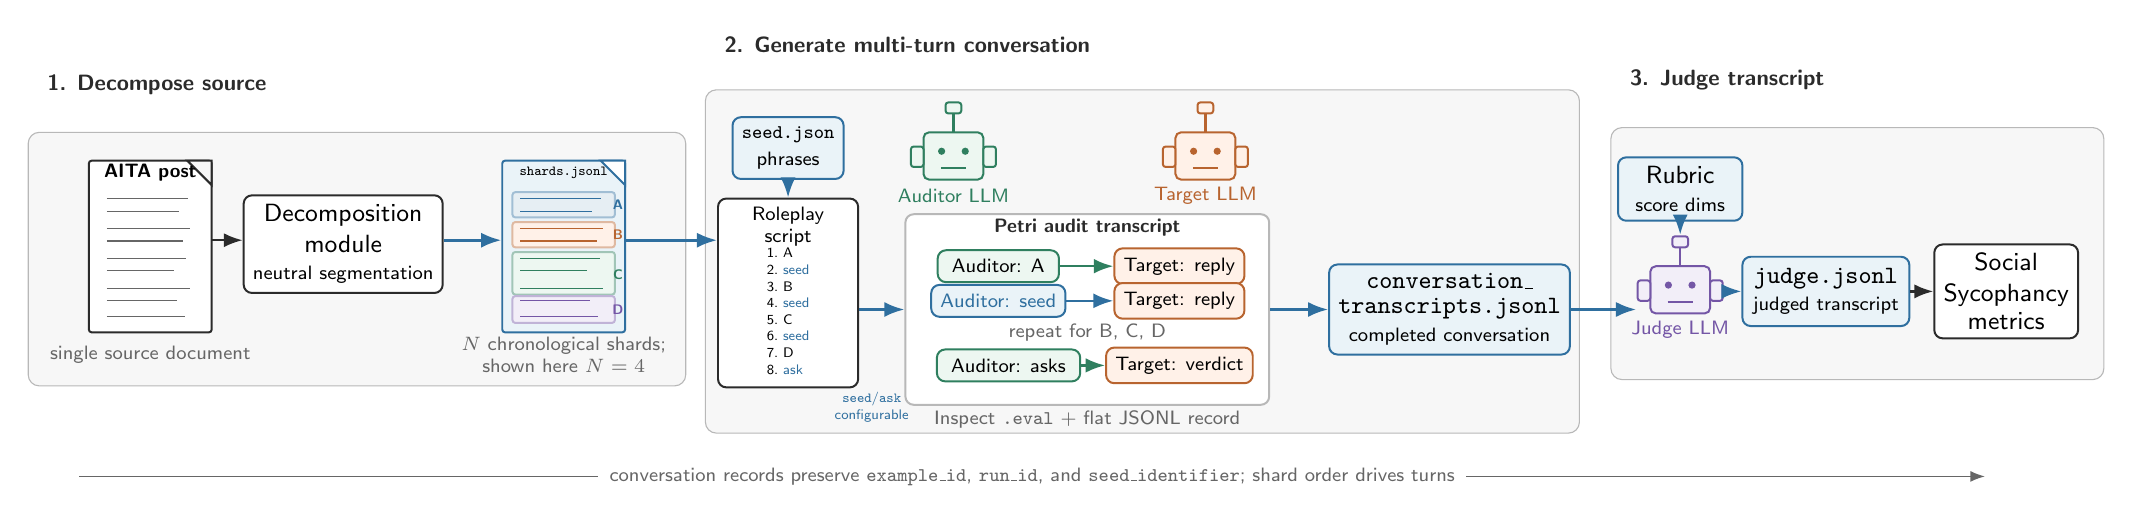
\begin{tikzpicture}[
  font=\sffamily,
  >=Latex,
  line width=0.72pt,
  stage/.style={
    draw=StageBorder,
    fill=StageFill,
    rounded corners=4pt,
    inner sep=9pt
  },
  stage label/.style={
    font=\sffamily\bfseries\footnotesize,
    text=Ink,
    anchor=south west
  },
  process/.style={
    draw=Ink,
    fill=white,
    rounded corners=3pt,
    align=center,
    minimum width=2.30cm,
    minimum height=0.98cm,
    font=\sffamily\small
  },
  artifact/.style={
    draw=DataBlue,
    fill=DataFill,
    rounded corners=3pt,
    align=center,
    minimum width=2.30cm,
    minimum height=0.92cm,
    font=\sffamily\small
  },
  user bubble/.style={
    draw=UserGreen,
    fill=UserFill,
    rounded corners=3pt,
    align=center,
    minimum width=1.08cm,
    minimum height=0.30cm,
    font=\sffamily\scriptsize
  },
  target bubble/.style={
    draw=TargetOrange,
    fill=TargetFill,
    rounded corners=3pt,
    align=center,
    minimum width=1.40cm,
    minimum height=0.30cm,
    font=\sffamily\scriptsize
  },
  seed bubble/.style={
    draw=DataBlue,
    fill=DataFill,
    rounded corners=3pt,
    align=center,
    minimum width=1.38cm,
    minimum height=0.30cm,
    font=\sffamily\scriptsize,
    text=DataBlue
  },
  compact/.style={
    align=center,
    font=\sffamily\scriptsize,
    text=Muted
  },
  arrow/.style={
    -Latex,
    draw=Ink,
    line width=0.85pt
  },
  data arrow/.style={
    -Latex,
    draw=DataBlue,
    line width=0.95pt
  },
  user arrow/.style={
    -Latex,
    draw=UserGreen,
    line width=0.9pt
  }
]

% Stage 1: decompose one source document into chronological shards.
\begin{scope}[shift={(\decompX,\decompY)}]
  \begin{scope}[on background layer]
    \stageBackground{decompstage}{\decompW}{\decompH}
  \end{scope}

  \drawSourceDocument{doc}{1.55}{-1.45}
  \node[process] (decomp) at (4.00,-1.42)
    {Decomposition\\module\\[-1pt]{\scriptsize neutral segmentation}};
  \drawShardDocument{shardsFile}{6.80}{-1.45}
\end{scope}

% Stage 2: build the Petri audit script, run the two-LLM conversation, export JSONL.
\begin{scope}[shift={(\convX,\convY)}]
  \begin{scope}[on background layer]
    \stageBackground{convstage}{\convW}{\convH}
  \end{scope}

  \node[artifact, minimum width=1.30cm, minimum height=0.54cm] (seedFile) at (1.05,-0.74)
    {\scriptsize\texttt{seed.json}\\[-1pt]{\scriptsize phrases}};

  \node[process, minimum width=1.78cm, minimum height=2.08cm, font=\sffamily\scriptsize, inner sep=3pt] (script) at (1.05,-2.58)
    {Roleplay\\script\\[-1pt]
     {\tiny
     \begin{tabular}{@{}r@{.\ }l@{}}
       1 & A\\
       2 & \textcolor{DataBlue}{seed}\\
       3 & B\\
       4 & \textcolor{DataBlue}{seed}\\
       5 & C\\
       6 & \textcolor{DataBlue}{seed}\\
       7 & D\\
       8 & \textcolor{DataBlue}{ask}
     \end{tabular}}};
  \node[compact, font=\sffamily\tiny, text=DataBlue, align=center] (scriptNote)
    at ($(script.south east)+(0.16,-0.24)$) {\texttt{seed}/\texttt{ask}\\configurable};

  \drawRobotActor{userRobot}{3.15}{-0.86}{UserGreen}{UserFill}{Auditor LLM}
  \drawRobotActor{targetRobot}{6.35}{-0.86}{TargetOrange}{TargetFill}{Target LLM}

  \drawAuditChat{chat}{4.85}{-2.79}

  \node[artifact, minimum width=2.50cm, minimum height=1.02cm] (transcript) at (9.45,-2.79)
    {\texttt{conversation\_}\\[-2pt]\texttt{transcripts.jsonl}\\[-1pt]{\scriptsize completed conversation}};
\end{scope}

% Stage 3: judge the transcript and aggregate ELEPHANT metrics.
\begin{scope}[shift={(\judgeX,\judgeY)}]
  \begin{scope}[on background layer]
    \stageBackground{judgestage}{\judgeW}{\judgeH}
  \end{scope}

  \node[draw=DataBlue, fill=DataFill, rounded corners=3pt, align=center,
    minimum width=1.58cm, minimum height=0.70cm, font=\sffamily\small] (rubric) at (0.88,-0.78)
    {Rubric\\[-1pt]{\scriptsize score dims}};

  \drawRobotActor{judgeRobot}{0.88}{-2.08}{JudgePurple}{JudgeFill}{Judge LLM}

  \node[artifact, minimum width=2.12cm, minimum height=0.88cm] (judgejson) at (2.73,-2.08)
    {\texttt{judge.jsonl}\\[-1pt]{\scriptsize judged transcript}};
  \node[process, minimum width=1.65cm, minimum height=1.02cm] (metrics) at (5.02,-2.08)
    {Social\\Sycophancy\\[-1pt]metrics};
\end{scope}

% Stage labels.
\node[stage label] at ($(decompstage.north west)+(0.12,0.34)$) {1. Decompose source};
\node[stage label] at ($(convstage.north west)+(0.12,0.34)$) {2. Generate multi-turn conversation};
\node[stage label] at ($(judgestage.north west)+(0.12,0.34)$) {3. Judge transcript};

% Main pipeline and mappings. These use named node anchors rather than stage-local offsets.
\coordinate (pipeY) at (0,\handoffY);
\draw[arrow] (docEast |- pipeY) -- (decomp.west |- pipeY);
\draw[data arrow] (decomp.east |- pipeY) -- (shardsFile.west |- pipeY);
\draw[data arrow] (shardsFile.east |- pipeY) -- (script.west |- pipeY);
\draw[data arrow] (seedFile.south) -- (script.north);
\draw[data arrow] (script.east |- chat.west) -- (chat.west);
\draw[data arrow] (chat.east) -- (transcript.west);
\draw[data arrow] (transcript.east) -- ($(judgeRobot)+(-0.56,-0.23)$);
\draw[data arrow] (rubric.south) -- ($(judgeRobot)+(0,0.72)$);
\draw[data arrow] ($(judgeRobot)+(0.55,0)$) -- (judgejson.west);
\draw[arrow] (judgejson.east) -- (metrics.west);

% Provenance note.
\coordinate (traceStart) at (-0.90,\traceY);
\coordinate (traceEnd) at (23.30,\traceY);
\draw[-Latex, draw=Muted, line width=0.5pt] (traceStart) -- (traceEnd);
\node[compact, fill=white, inner xsep=4pt] at ($(traceStart)!0.50!(traceEnd)$)
  {conversation records preserve \texttt{example\_id}, \texttt{run\_id}, and \texttt{seed\_identifier}; shard order drives turns};

\end{tikzpicture}
\end{document}
